\documentclass[11pt,a4paper]{article}
\usepackage[utf8]{inputenc}
\usepackage[T1]{fontenc}
\usepackage[a4paper,margin=2.4cm]{geometry}
\usepackage{amsmath,amssymb,mathtools}
\usepackage{physics}
\usepackage{siunitx}
\usepackage{graphicx}
\usepackage{booktabs}
\usepackage{xcolor}
\usepackage{hyperref}
\hypersetup{colorlinks=true, linkcolor=blue!50!black,
            citecolor=blue!50!black, urlcolor=blue!50!black}
\usepackage{cleveref}
\usepackage{algorithm}
\usepackage{algpseudocode}
\usepackage{tcolorbox}
\tcbuselibrary{breakable}
\usepackage{caption}
\captionsetup{font=small, labelfont=bf}

\newcommand{\Eg}{E_\gamma}
\newcommand{\Egp}{E_\gamma'}
\newcommand{\me}{m_e c^2}
\newcommand{\re}{r_e}
\newcommand{\Qbb}{Q_{\beta\beta}}
\newcommand{\zeronubb}{0\nu\beta\beta}
\newcommand{\eps}{\varepsilon}
\newcommand{\sigKN}{\sigma_{\rm KN}}
\newcommand{\Tcut}{T_e^{\rm cut}}
\newcommand{\kmin}{k_{\min}}
\newcommand{\Egcut}{\Eg^{\rm cut}}

\newtcolorbox{remarkbox}{colback=blue!4!white, colframe=blue!50!black,
  sharp corners, fonttitle=\bfseries, title={Remark}, breakable}
\newtcolorbox{cautionbox}{colback=red!4!white, colframe=red!60!black,
  sharp corners, fonttitle=\bfseries, title={Caution}, breakable}

\title{\bfseries A Pedagogical Monte Carlo for Photons and Electrons \\
       in a Liquid Xenon Calorimeter \\[6pt]
       \large with application to single-site / multi-site
       discrimination near $\Qbb$}
\author{}
\date{\today}

\begin{document}
\maketitle

\begin{abstract}\noindent
We describe, in tutorial style, a complete electromagnetic Monte Carlo
adequate for the simulation of the response of a large liquid-xenon
($\rm LXe$) calorimeter to MeV-scale photons of the kind encountered
in neutrinoless double-beta decay searches. The algorithm treats
Compton scattering, pair production and photoelectric absorption as
discrete photon processes, and transports electrons and positrons
step-by-step using NIST ESTAR stopping powers and explicit
bremsstrahlung sampling. The code is structured as a small set of
independent modules; numerical anchors come from authoritative NIST
tables (XCOM for photon cross sections, ESTAR for electron stopping
powers) and from the Geant4-distributed Sandia photoelectric
coefficients. The manual discusses the physics and the statistical
sampling methods, and includes a critical comparison with the
corresponding {\sc Geant4} models. A working Python implementation
and the data files are distributed alongside this document.
\end{abstract}

\tableofcontents
\bigskip\hrule\bigskip

\section{Introduction and motivation}\label{sec:intro}

This is a self-contained description of a custom electromagnetic
Monte Carlo for the interaction of MeV-scale $\gamma$-rays with a
large liquid-xenon calorimeter. It is the workhorse for sensitivity
studies of neutrinoless double-beta decay ($\zeronubb$) experiments
using $\rm{}^{136}Xe$~\cite{LZ,nEXO,EXO200,NEXT}; we feel that
working through every step from first principles, rather than
treating {\sc Geant4}~\cite{G4-1,G4-PRM} as an oracle, is one of the
most rewarding pedagogical exercises in computational particle
physics one can offer to a graduate student.

\subsection{The $\zeronubb$ search and the SS/MS classifier}

The $\zeronubb$ signal in $\rm{}^{136}Xe$ is two electrons sharing
the $Q$-value of the decay,
\begin{equation}
  \Qbb \;=\; \SI{2.4578}{\MeV}\,.
\end{equation}
Because the two electrons have a combined CSDA range below
\SI{1}{cm} in $\rm LXe$, the signal is a single, localized energy
deposit (\emph{single-site}, SS) of energy $\Qbb$. The dominant
backgrounds in the region of interest (ROI) are external
$\gamma$-rays from the $\rm{}^{238}U$ and $\rm{}^{232}Th$ chains:
\begin{align*}
  \rm{}^{214}Bi\,&: \;\Eg=\SI{2.4476}{\MeV} \quad(\text{essentially in ROI}),\\
  \rm{}^{208}Tl\,&: \;\Eg=\SI{2.6145}{\MeV} \quad(\text{above ROI}).
\end{align*}
A $\gamma$-ray of energy above the ROI can deposit precisely $\Qbb$
via Compton or photoelectric processes if part of the energy
escapes; conversely a $\gamma$-ray very close to the ROI can be
wholly absorbed and fall into the window. In both cases the event
is reconstructed as SS only if the spatial extent of the energy
deposition is small compared to the detector resolution. In a
typical large LXe TPC the only relevant resolution is along the
drift direction $z$,
\begin{equation}
  \Delta z \;\approx\; \SI{3}{mm}\,,
\end{equation}
and the SS / MS classifier separates events whose secondary energy
deposits lie within $\Delta z$ of the primary deposit (SS) from
those that do not (MS).

\subsection{What this manual covers}

\Cref{fig:topology} captures the central question. A naive MC that
samples only the Klein--Nishina formula and treats each Compton
vertex as a point energy deposit (left) misses two effects of
comparable magnitude:
\begin{enumerate}\itemsep=0pt
  \item the \emph{electron range}~--~MeV electrons in $\rm LXe$
        have ranges of several mm, smearing the energy deposit
        along an electron track;
  \item the \emph{bremsstrahlung} emission of those electrons,
        which produces secondary photons that may travel several
        cm before depositing elsewhere.
\end{enumerate}
The first effect can {\em bridge} two nearby Compton vertices and
turn an MS event into an SS event; the second can {\em split} an
SS-looking event into a multi-site one. In addition, the
\emph{photoelectric} channel~--~though small in absolute branching
($\sim 2\%$ at our energies)~--~deposits the full primary energy
at a single point and is therefore the most dangerous SS-mimic
mode; we treat it carefully in \Cref{sec:phot,sec:ssmimic}.

\begin{figure}[ht]
  \centering
  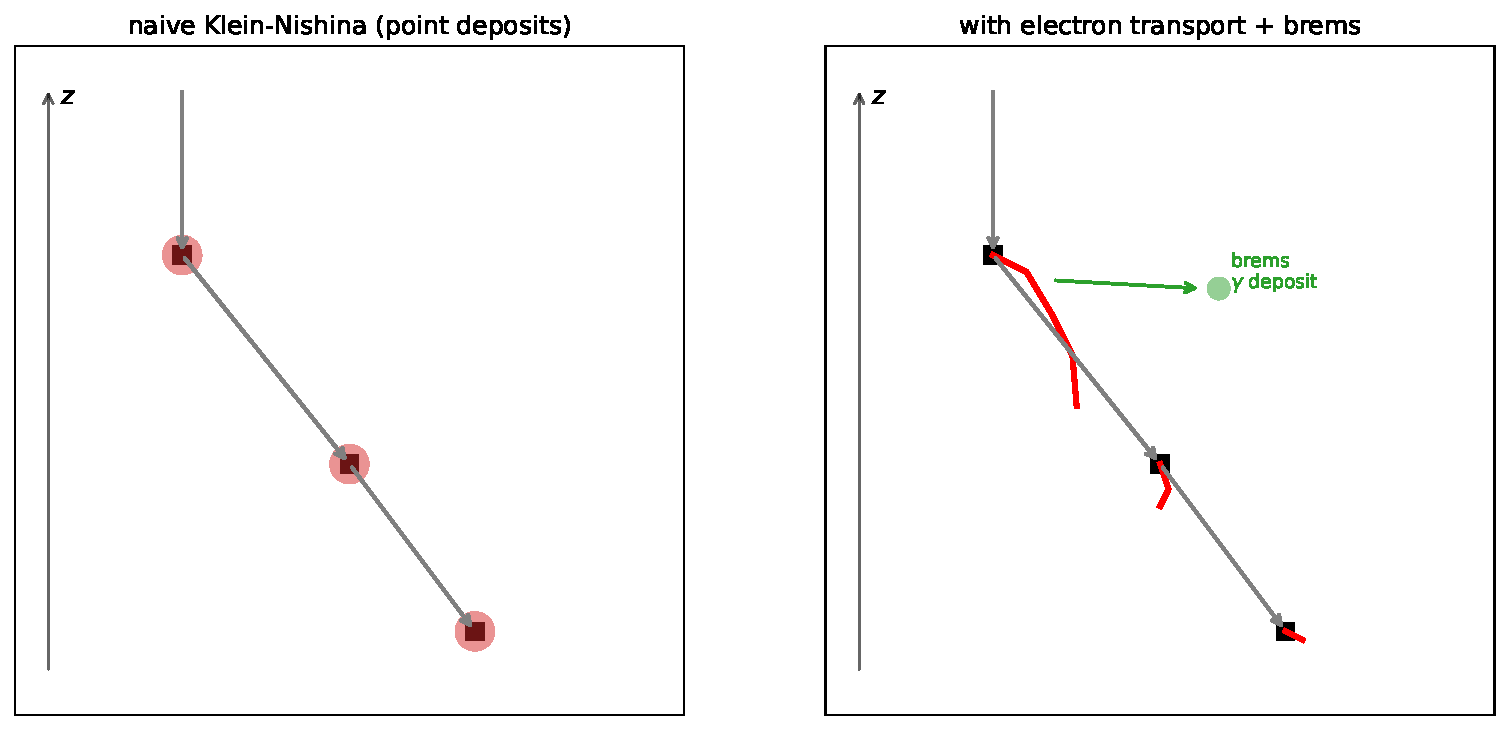
\includegraphics[width=\textwidth]{figs/topology_schematic.pdf}
  \caption{Cartoon of a $\gamma$-ray event in $\rm LXe$.
  \emph{Left:} naive Klein--Nishina-only treatment (red blobs at
  Compton vertices). \emph{Right:} the same event with electron
  transport and explicit bremsstrahlung (red lines: electron
  tracks; green: a brems photon depositing far from the vertex).}
  \label{fig:topology}
\end{figure}

\subsection{Approach: analytic formulas, NIST anchors}

Pedagogy demands that every cross section be an explicit analytic
formula; production-grade numbers want \emph{tabulated} cross
sections from authoritative compilations. This manual takes a
hybrid approach:
\begin{itemize}\itemsep=0pt
  \item Each physical process is presented as an analytic formula
        with full derivation cues, so that the reader sees what
        is being computed.
  \item Numerical results in tables and figures are anchored to
        NIST XCOM~\cite{NIST-XCOM} for photon cross sections and
        NIST ESTAR~\cite{NIST-ESTAR} for electron stopping
        powers. The Sandia photoelectric
        parameterization~\cite{BiggsLighthill,G4-PRM} provides an
        analytic formula valid below \SI{500}{keV}.
  \item Every figure shows lines (analytic formulas) overlaid
        with markers (NIST data). Where the two diverge~--~as
        for Sandia photoelectric above \SI{500}{keV}~--~we say
        so explicitly.
\end{itemize}

\section{Photon interactions in xenon: an overview}
\label{sec:photonphys}

A $\gamma$-ray traverses a medium freely between discrete
interactions whose mean free path is
\begin{equation}
  \lambda(\Eg) = \frac{1}{n_{\rm at}\,\sigma_{\rm tot}(\Eg)},
  \qquad
  n_{\rm at} = \rho N_A / A.
\end{equation}
For $\rm LXe$ at \SI{165}{K}, $\rho=\SI{2.953}{g/cm^3}$, $A=131.293$,
$Z=54$, hence $n_{\rm at}=\SI{1.354e22}{cm^{-3}}$. The total cross
section is the sum of three contributions:
\begin{equation}
  \sigma_{\rm tot} = \sigma_{\rm C} + \sigma_{\rm P} + \sigma_{\rm Ph},
\end{equation}
Compton (incoherent), pair production, and photoelectric. The
Rayleigh (coherent) channel is omitted because it deposits no
energy.

\begin{figure}[ht]
  \centering
  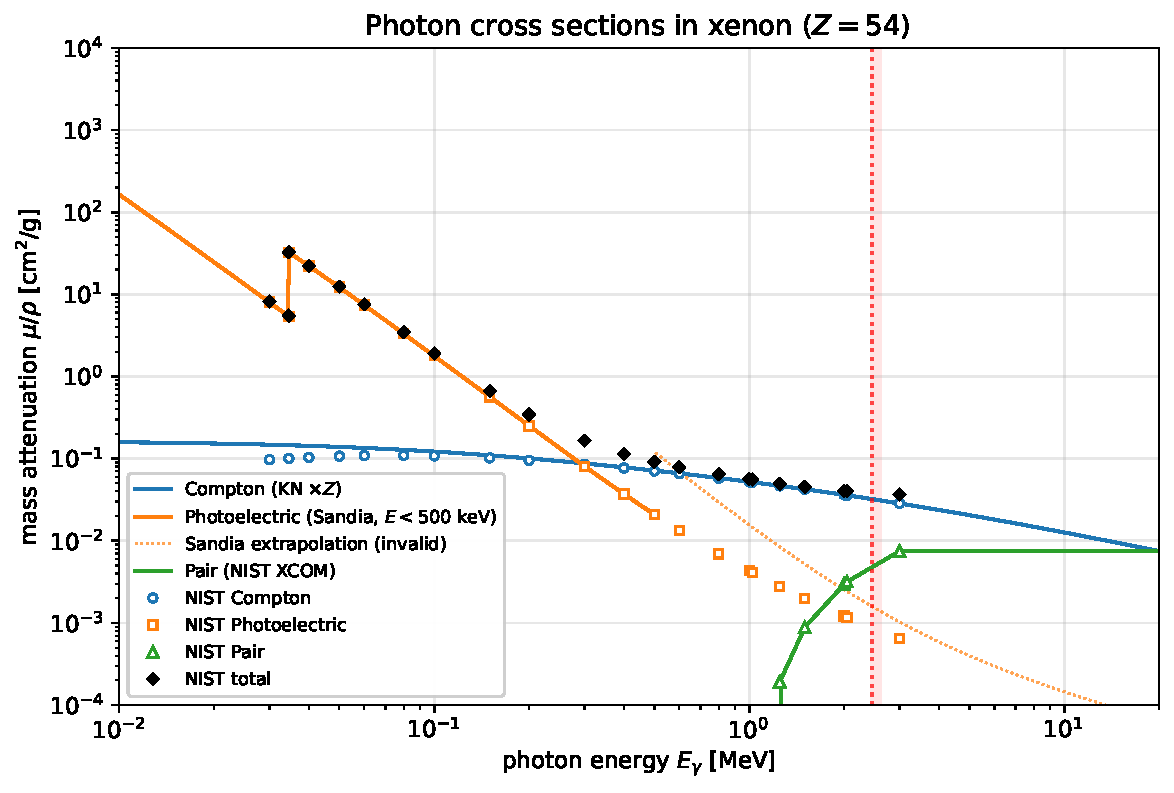
\includegraphics[width=0.9\textwidth]{figs/xsec_xe.pdf}
  \caption{Photon mass attenuation $\mu/\rho$ in xenon.
  Lines: analytic formulas (Klein--Nishina $\times Z$ for
  Compton, Bethe-Heitler integrated for pair, Sandia for
  photoelectric below \SI{500}{keV}; the dotted orange line is
  Sandia's high-energy interval, which extrapolates badly).
  Markers: NIST XCOM~\cite{NIST-XCOM}. Red band: ROI window.}
  \label{fig:xsec}
\end{figure}

The branching fractions and mean free paths near $\Qbb$ are
summarized in \Cref{tab:branching}, all from NIST
XCOM~\cite{NIST-XCOM}.

\begin{table}[ht]
\centering
\caption{Branching fractions and mfp in $\rm LXe$ at the energies
of interest, from NIST XCOM~\cite{NIST-XCOM}.}
\label{tab:branching}
\begin{tabular}{lccccc}
\toprule
$\gamma$ source & $\Eg$ [MeV] & $\sigma_{\rm C}/\sigma_{\rm tot}$
& $\sigma_{\rm P}/\sigma_{\rm tot}$ & $\sigma_{\rm Ph}/\sigma_{\rm tot}$
& $\lambda$ [cm] \\
\midrule
$\rm{}^{214}Bi$ line & 2.448 & 0.851 & 0.125 & 0.023 & 8.81 \\
$\Qbb$               & 2.458 & 0.850 & 0.127 & 0.023 & 8.81 \\
$\rm{}^{208}Tl$ line & 2.615 & 0.831 & 0.148 & 0.021 & 8.94 \\
\bottomrule
\end{tabular}
\end{table}

\begin{cautionbox}
An earlier draft of this manual stated ``few-per-mille'' for the
photoelectric branching at our energies. \textbf{This was wrong
by a factor of order 30}: the correct value from NIST XCOM is
$\approx 2.3\%$ at $\Qbb$. The implications for SS background
estimation are discussed in \Cref{sec:ssmimic}.
\end{cautionbox}

\begin{figure}[ht]
  \centering
  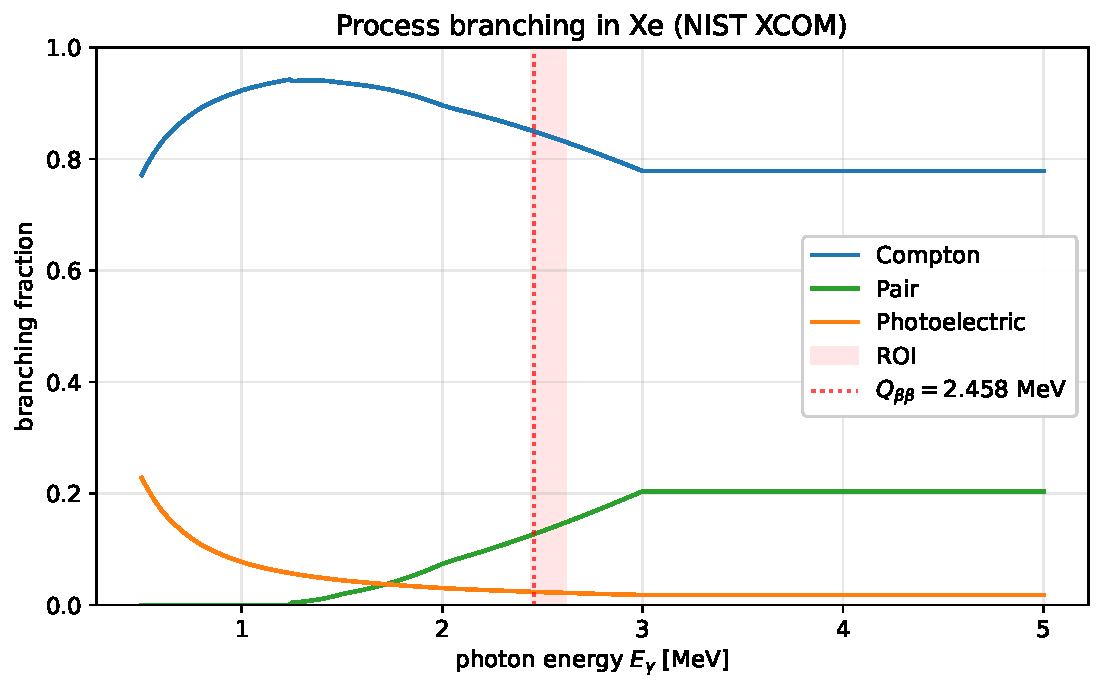
\includegraphics[width=0.78\textwidth]{figs/branching_xe.pdf}
  \caption{Process branching in xenon (NIST XCOM). Compton
  dominates the entire ROI region.}
  \label{fig:branching}
\end{figure}


\section{Compton scattering}\label{sec:compton}

\subsection{Kinematics and the Klein-Nishina cross section}

We treat the bound atomic electron as free and at rest~--~the
\emph{free-electron approximation}, valid for $\Eg \gg E_K =
\SI{34.6}{keV}$. Energy-momentum conservation gives the Compton
relation
\begin{equation}
  \Egp = \frac{\Eg}{1 + (\Eg/\me)(1-\cos\theta)},
  \qquad
  T_e = \Eg - \Egp,
  \label{eq:compton}
\end{equation}
where $\theta$ is the photon scattering angle. The maximum kinetic
energy is delivered at $\theta=\pi$,
\begin{equation}
  T_e^{\max}=\Eg\,\frac{2\Eg/\me}{1+2\Eg/\me}.
\end{equation}
For $\rm{}^{208}Tl$, $T_e^{\max}=\SI{2.382}{MeV}$ (the Compton edge).

The differential cross section per electron is the Klein-Nishina
formula~\cite{KleinNishina}:
\begin{equation}
  \dv{\sigKN}{\Omega}(\theta;\Eg)
  = \frac{1}{2}\re^2\Bigl(\frac{\Egp}{\Eg}\Bigr)^{\!2}
    \Bigl[\frac{\Eg}{\Egp} + \frac{\Egp}{\Eg} - \sin^2\theta\Bigr],
  \label{eq:KN-diff}
\end{equation}
with the integrated form
\begin{equation}
  \sigKN(\Eg) = 2\pi\re^2\!\left[
    \frac{1+\eta}{\eta^2}\!
    \left(\frac{2(1+\eta)}{1+2\eta}-\frac{\ln(1+2\eta)}{\eta}\right)
    +\frac{\ln(1+2\eta)}{2\eta}-\frac{1+3\eta}{(1+2\eta)^2}
    \right],
\end{equation}
$\eta=\Eg/\me$. The atomic cross section is
$\sigma_{\rm C}\simeq Z\,\sigKN$ above the K-edge.

\begin{figure}[ht]
\centering
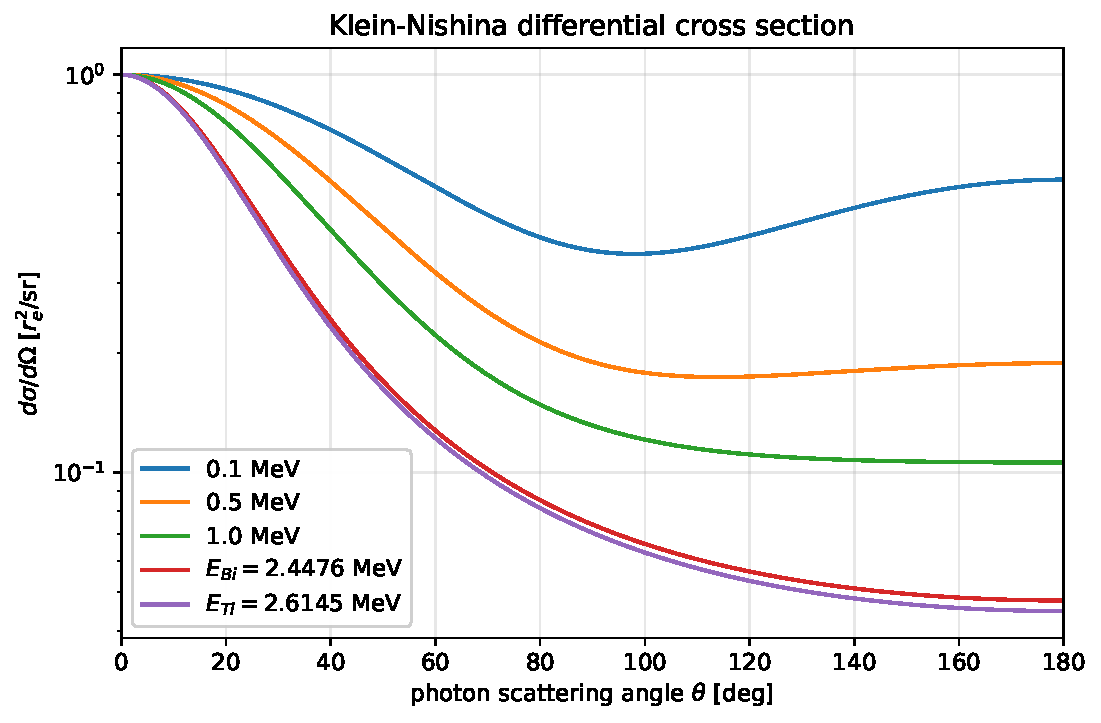
\includegraphics[width=0.72\textwidth]{figs/kn_diff.pdf}
\caption{Klein-Nishina differential cross section. As $\Eg$
increases the distribution becomes increasingly forward peaked.}
\label{fig:KN_diff}
\end{figure}

\begin{figure}[ht]
\centering
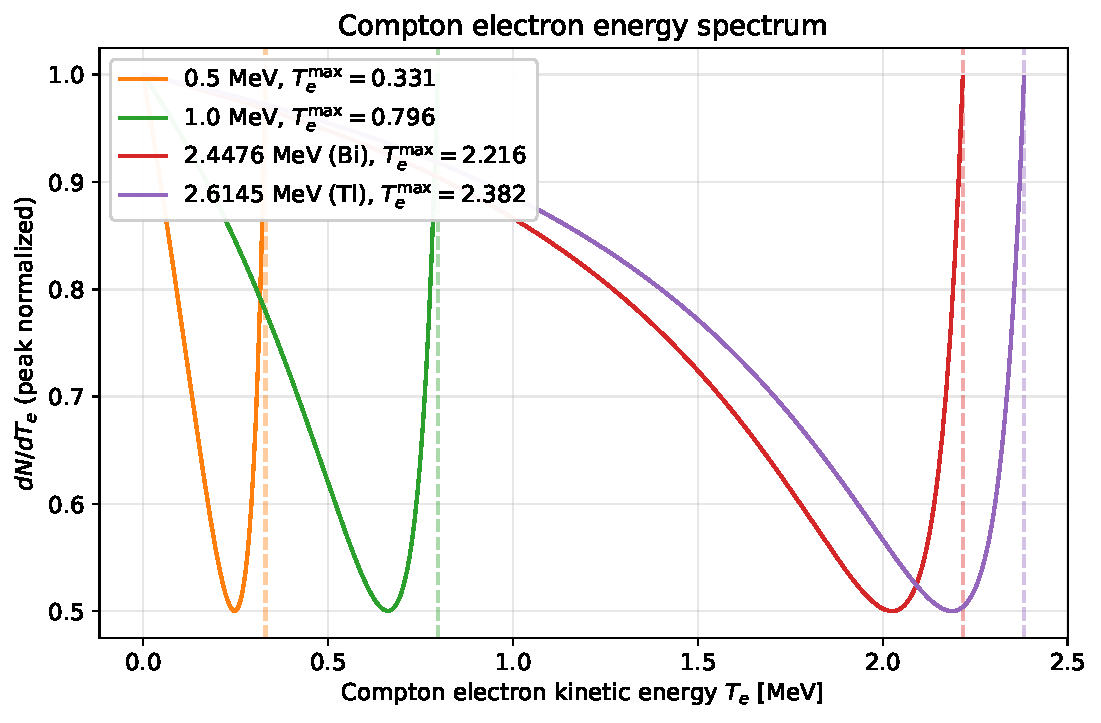
\includegraphics[width=0.72\textwidth]{figs/compton_electron_spectrum.pdf}
\caption{Compton-electron kinetic-energy spectrum.}
\label{fig:Te_spec}
\end{figure}

\subsection{Recoil electron direction}

From momentum conservation in the lab frame,
\begin{equation}
  \cos\phi_e = \frac{1+\Eg/\me}{\sqrt{1+2\Eg/\me}}\,
              \tan(\theta/2).
\end{equation}
Equivalently, $\vec p_e=\vec p_\gamma-\vec p_{\gamma'}$ with the
electron azimuth opposite that of the scattered photon.

\section{Pair production}\label{sec:pair}

For $\Eg > 2\me=\SI{1.022}{MeV}$ the photon can convert into an
$e^+e^-$ pair in the field of a nucleus. The differential cross
section in the Bethe-Heitler approximation, with screening and the
Coulomb correction~\cite{G4-PRM,Hubbell1980}:
\begin{multline}
\dv{\sigma_{\rm P}}{\eps}(Z,\eps;\Eg)
  = \alpha\re^2 Z[Z+\xi(Z)] \\
\times\Bigl\{
  [\eps^2+(1-\eps)^2]
  [\Phi_1(\delta)-\tfrac{1}{2}F(Z)]
  + \tfrac{2}{3}\eps(1-\eps)
  [\Phi_2(\delta)-\tfrac{1}{2}F(Z)]
\Bigr\},
\label{eq:BH-diff}
\end{multline}
where $\eps=E_+/\Eg$ and the screening parameter is
\(\delta(\eps) = (136/Z^{1/3})(\me/\Eg)/[\eps(1-\eps)]\).
The screening functions are tabulated piecewise:
\begin{align}
  \delta\le 1\!:\;&\Phi_1=20.867-3.242\delta+0.625\delta^2,\;
  \Phi_2=20.209-1.930\delta-0.086\delta^2,\\
  \delta>1\!:\;&\Phi_1=\Phi_2=21.12-4.184\,\ln(\delta+0.952),
\end{align}
$F(Z)=\frac{8}{3}\ln Z$, $\xi(Z)=\ln(1440/Z^{2/3})/[\ln(183/Z^{1/3})-f_c]$.
The kinematic limits are $\eps_0=\me/\Eg\le\eps\le 1-\eps_0$.

\begin{remarkbox}
At $\Eg<\SI{2}{MeV}$ the differential is essentially constant in
$\eps$ and the energy split can be sampled \emph{uniformly} on
$[\eps_0,1-\eps_0]$ with no rejection. For our two backgrounds at
2.448 and 2.615 MeV we are just above this regime; uniform sampling
is correct to $\sim 1\%$ and is adopted in our simulation.
\end{remarkbox}

\subsection{Polar angles of the leptons}

The $e^+$ and $e^-$ are emitted forward, with characteristic angle
$\me/E_\pm$. We use the parameterization of \cite{Urban1993,G4-PRM}:
\begin{equation}
  f(u) = \frac{9a^2}{9+d}(u\,e^{-au} + d\,u\,e^{-3au}),
  \quad a=\tfrac{5}{8},\; d=27,\;
  \theta_\pm = (\me/E_\pm)\,u .
\end{equation}
The two leptons are coplanar with the incoming photon.

\subsection{Positron annihilation}\label{sec:annih}

A positron loses energy by collisions and bremsstrahlung in
exactly the same way as an electron of the same kinetic energy.
When $T_+ < \Tcut$ we treat it as if it stops in place and
annihilates with an atomic electron, producing two
$\me=\SI{511}{keV}$ photons back-to-back and isotropic in the
laboratory frame. Both photons are pushed onto the photon stack
and propagated as new gammas. We neglect in-flight annihilation
(\(\sim 1\%\)) and three-photon (ortho-Ps) decay
(\(1/372\)).

\section{Photoelectric absorption}\label{sec:phot}

For our energies the photoelectric channel carries
\textbf{about 2\%} of the total cross section in xenon
(\Cref{tab:branching}). It is the smallest of the three channels
but, as we shall argue in \Cref{sec:ssmimic}, also the single most
dangerous mode for SS-faking ROI background events~--~because it
deposits the full primary energy at one point with $100\%$
probability of being SS.

In addition, secondary low-energy photons (from the brems tail or
the Compton chain) end their lives photoelectrically: above the
K-edge of xenon, $\sigma_{\rm Ph}\propto Z^{4\text{-}5}/\Eg^{3.5}$
wins below $\sim\SI{500}{keV}$. The resulting K-shell vacancy
has a $\SI{29.78}{keV}$ fluorescence transition with branching
$\omega_K=0.89$~\cite{Krause1979}, producing a small additional
photon that travels $\sim\SI{0.5}{mm}$ in $\rm LXe$.

\subsection{The Sandia parameterization}

The Sandia parameterization (Biggs \& Lighthill
1990~\cite{BiggsLighthill}) provides analytic coefficients for the
photoelectric cross section as a piecewise quartic in $1/E$:
\begin{equation}
  \frac{\sigma_{\rm Ph}}{\rho}\,[\text{cm}^2/\text{g}]
  = \frac{a_1}{E} + \frac{a_2}{E^2} + \frac{a_3}{E^3} + \frac{a_4}{E^4},
  \qquad E\;\text{in keV}\,,
  \label{eq:Sandia}
\end{equation}
with $\{a_i\}$ tabulated in energy intervals delimited by the
absorption edges. The full table for Xe (13 intervals from \SI{10}{eV}
to above \SI{500}{keV}) is included in the data files
distributed with this manual~\cite{G4-PRM}.

\begin{cautionbox}
\textbf{Sandia validity domain.} The Sandia coefficients for Xe
agree with NIST XCOM to $\sim 1\%$ \emph{below \SI{500}{keV}}.
The high-energy interval $[500\,\text{keV},\,\infty)$ is fit to a
small set of points and \emph{extrapolates badly} at MeV energies:
at $\Eg=\SI{1}{MeV}$ Sandia gives $1.6\times 10^{-2}\,\text{cm}^2/\text{g}$,
NIST XCOM gives $4.3\times 10^{-3}\,\text{cm}^2/\text{g}$ (off by
$3.6\times$); at $\Eg=\SI{3}{MeV}$ the discrepancy is still
$1.6\times$. \Cref{fig:sandia_vs_nist} shows this graphically.
\textbf{In our simulation we therefore use Sandia for
$\Eg<\SI{500}{keV}$ and interpolate NIST XCOM above.} This dual
approach mirrors that of modern codes like {\sc Geant4}, which
uses the Livermore EPDL97 tables in this regime
(\verb|G4LivermorePhotoElectricModel|).
\end{cautionbox}

\begin{figure}[ht]
\centering
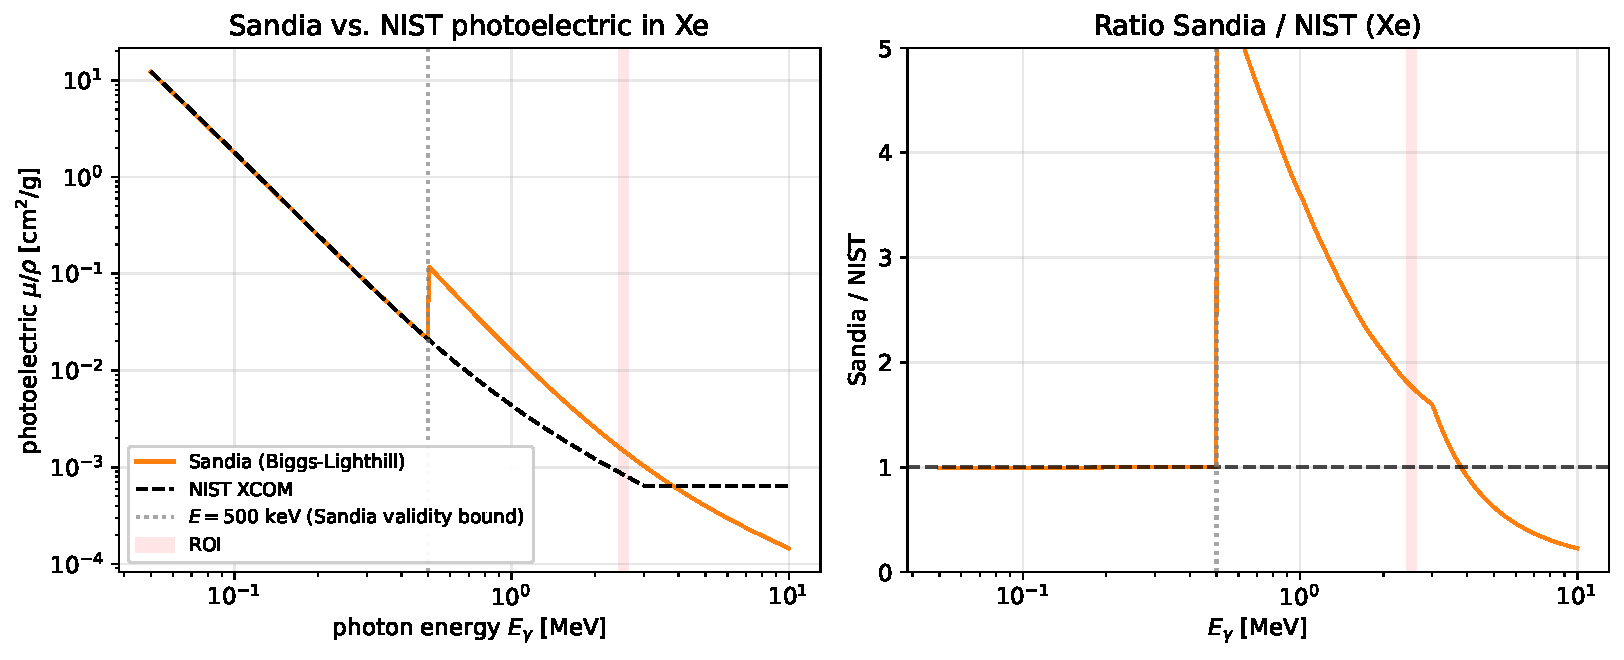
\includegraphics[width=\textwidth]{figs/sandia_vs_nist.pdf}
\caption{Comparison of the Sandia parameterization with NIST XCOM
for photoelectric absorption in Xe. Below \SI{500}{keV} the two
agree to $\sim 1\%$; above, Sandia extrapolates poorly. The ratio
panel makes the discrepancy visible across the ROI region.}
\label{fig:sandia_vs_nist}
\end{figure}

\subsection{Final state and atomic relaxation}

The photoelectron is ejected with $T_e=\Eg-E_{\rm shell}$.
Above the K-edge, the K-shell takes $\sim 80\%$ of all events,
the L-shell $\sim 15\%$, the rest going to higher
shells~\cite{G4-PRM}. The polar angle is sampled from the
zeroth-order Sauter distribution
\begin{equation}
  \dv{\sigma}{\cos\theta_e} \propto
  \frac{\sin^2\theta_e}{(1-\beta\cos\theta_e)^4}\,.
\end{equation}

The K-shell vacancy is filled either by emission of a $K_\alpha$
photon ($\SI{29.78}{keV}$, probability $\omega_K=0.89$) or by
emission of an Auger electron ($T_{\rm Auger}\!\approx\!E_K-2E_L
\!\approx\!\SI{24.5}{keV}$, probability $1-\omega_K$). The Auger
electron is deposited locally; the fluorescence photon is pushed
onto the photon stack. For L- and higher shells we deposit the
binding energy locally (their fluorescence is below the photon
threshold).


\section{Energy loss of electrons and positrons}\label{sec:edE}

A charged lepton in $\rm LXe$ at our energies loses energy mostly
by ionization and to a smaller (but non-negligible) extent by
bremsstrahlung. We treat ionization as a continuous, deterministic
energy loss and bremsstrahlung as a discrete process whenever the
photon is hard enough to be relevant for the SS/MS classifier.

\subsection{Mass collision stopping power}

For electrons, the Berger-Seltzer
formula~\cite{ICRU37,Berger1964} (M\o{}ller cross section for
indistinguishable identical particles):
\begin{equation}
\boxed{\;
  \frac{1}{\rho}\dv{E}{x}\bigg|_{\rm coll}
  = \frac{K}{2}\frac{Z}{A}\frac{1}{\beta^2}
   \!\left[
     \ln\frac{\tau^2(\tau+2)}{2(I/\me)^2}
     + F^{-}(\tau) - \delta
   \right]
\;}
\end{equation}
with $\tau=T/\me$, $\beta=v/c$, $I=\SI{482}{eV}$ for xenon,
$K=4\pi N_A\re^2\me=\SI{0.30707}{MeV\,cm^2/g}$, and
\begin{equation}
  F^-(\tau) = 1-\beta^2 +\frac{\tau^2/8 - (2\tau+1)\ln 2}{(\tau+1)^2}.
\end{equation}
The density-effect correction $\delta$ is $<2\%$ at our energies
in $\rm LXe$ and is set to zero. Direct calculation matches NIST
ESTAR for elemental Xe to $<1\%$ (verified at $T=\SI{1}{MeV}$:
formula gives 1.122, ESTAR gives 1.122 MeV cm$^2$/g).

\subsection{Mass radiative stopping power}

The radiative loss is dominated by bremsstrahlung. In the Tsai
complete-screening form~\cite{Tsai1974}:
\begin{equation}
  \frac{1}{\rho}\dv{E}{x}\bigg|_{\rm rad}
  \simeq 4\,\alpha\,\frac{N_A}{A}\,Z(Z+1)\,\re^2\,
        (T+\me)\, L_{\rm rad},
  \quad
  L_{\rm rad}=\ln(183/Z^{1/3})-f_c(Z).
  \label{eq:rad-stop}
\end{equation}
The radiative \emph{fraction} of the total stopping power in xenon
rises from \SI{0.7}{\percent} at $T=\SI{0.05}{MeV}$ to
\SI{14}{\percent} at $T=\SI{2.4}{MeV}$~--~much larger than may
appear at first glance, and a key source of MS-like signatures in
the SS/MS classifier. \Cref{fig:stop-range} compares NIST ESTAR
values with our analytic formulas, and shows the CSDA range. The
range crosses $\Delta z=\SI{3}{mm}$ at $T\!\sim\!\SI{1.1}{MeV}$.

\begin{figure}[ht]
\centering
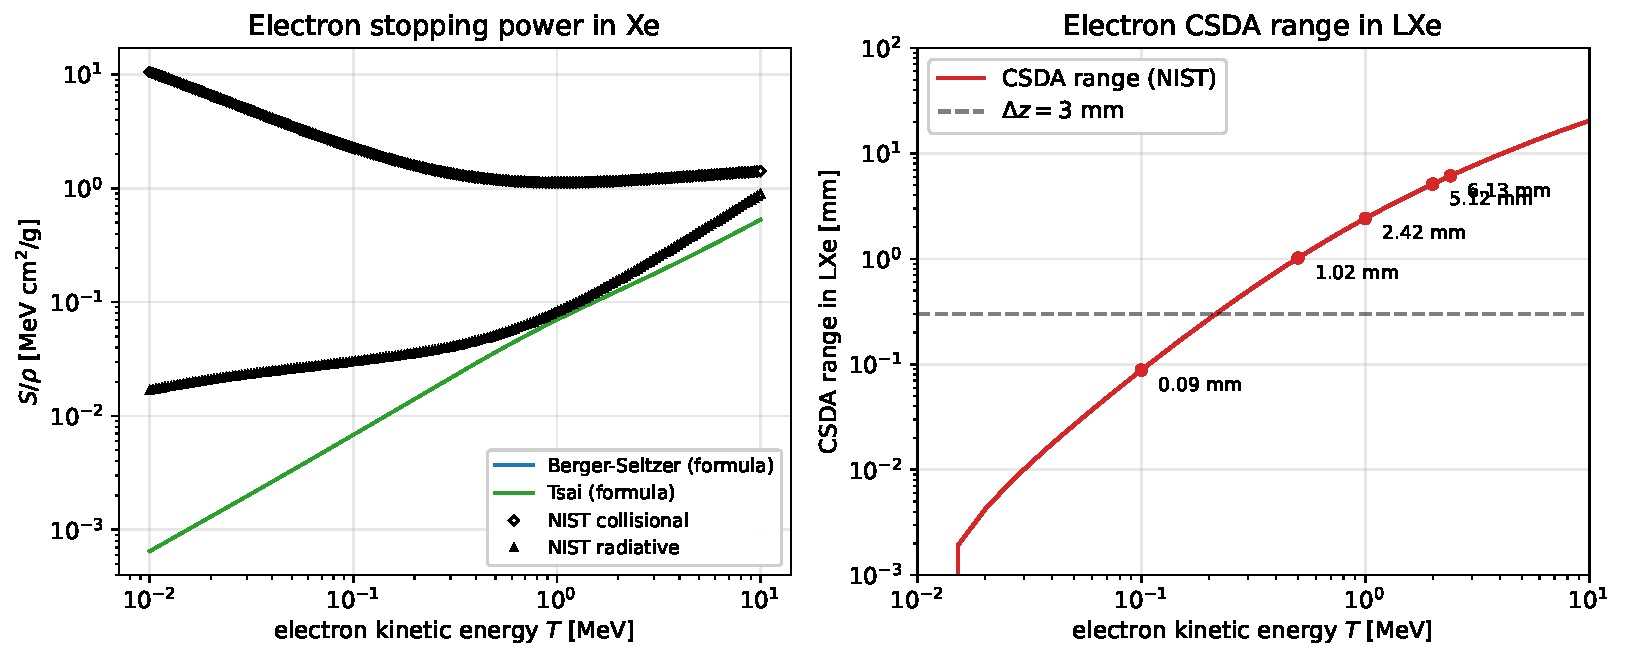
\includegraphics[width=\textwidth]{figs/stopping_range_xe.pdf}
\caption{\emph{Left:} mass collision and radiative stopping power
for electrons in xenon. Lines: analytic formulas (Berger-Seltzer,
Tsai). Markers: NIST ESTAR~\cite{NIST-ESTAR}. The Berger-Seltzer
formula reproduces ESTAR collisional values exactly (markers
overlay the line). The Tsai radiative formula underestimates
ESTAR by $\sim 15\%$; we therefore use ESTAR values directly in
the simulation. \emph{Right:} CSDA range in $\rm LXe$, computed
by integration of $1/S_{\rm tot}$ over ESTAR data. Dashed line:
$\Delta z=\SI{3}{mm}$ resolution.}
\label{fig:stop-range}
\end{figure}

\Cref{tab:range} gives quantitative values from NIST ESTAR.

\begin{table}[ht]
\centering
\caption{Electron stopping power and CSDA range in liquid xenon
($\rho=\SI{2.953}{g/cm^3}$), from NIST ESTAR~\cite{NIST-ESTAR}.
The ``rad\%'' column is the radiative fraction of total stopping
power, $S_{\rm rad}/(S_{\rm col}+S_{\rm rad})$.}
\label{tab:range}
\begin{tabular}{cccccc}
\toprule
$T$ [MeV] & $S_{\rm col}/\rho$ & $S_{\rm rad}/\rho$ &
$S_{\rm tot}/\rho$ & rad\% & $R_{\rm LXe}$ [mm] \\
          & [MeV cm$^2$/g]     & [MeV cm$^2$/g]     &
[MeV cm$^2$/g]     &       &                     \\
\midrule
0.05 & 3.513 & 0.026 & 3.539 & 0.7 & 0.027 \\
0.10 & 2.267 & 0.030 & 2.298 & 1.3 & 0.088 \\
0.25 & 1.445 & 0.038 & 1.483 & 2.6 & 0.378 \\
0.50 & 1.192 & 0.051 & 1.243 & 4.1 & 1.016 \\
1.00 & 1.122 & 0.082 & 1.204 & 6.8 & 2.418 \\
1.50 & 1.135 & 0.118 & 1.253 & 9.4 & 3.799 \\
2.00 & 1.160 & 0.156 & 1.316 & 11.8 & 5.118 \\
2.40 & 1.181 & 0.188 & 1.369 & 13.7 & 6.127 \\
3.00 & 1.211 & 0.237 & 1.448 & 16.4 & 7.570 \\
\bottomrule
\end{tabular}
\end{table}

\begin{remarkbox}
\textbf{Bragg behaviour.} The collisional stopping power has a
broad minimum near $T\!\simeq\!\SI{1}{MeV}$ and rises by roughly
a factor of $3$ as the electron slows from \SI{0.5}{MeV} to
\SI{0.05}{MeV}. The radiative component falls monotonically with
$T$. Total $\dd E/\dd x$ is thus back-loaded along an electron
track: more energy is deposited near the end. This Bragg-like
behaviour is naturally captured if the simulation steps the
electron in small increments, computing $\dd E/\dd x$ at each
step from the local kinetic energy~--~no separate Bragg-curve
model is needed.
\end{remarkbox}

\subsection{Multiple scattering, $\delta$-rays, fluctuations}
\label{sec:omitted-electron}

We do not include angular multiple scattering, $\delta$-ray
production, or energy-loss straggling. The justification, for our
SS/MS application:

\textbf{Multiple scattering.} The actual electron path is
tortuous. The error from drawing a straight CSDA segment is dominated
by fluctuations and is at most a few tens of \% on the SS-fraction
estimate, well below other systematics.

\textbf{$\delta$-rays.} A $\delta$-ray of $T'>\SI{50}{keV}$ at
MeV electron energy has range below \SI{50}{\micro\m} in $\rm LXe$,
far below $\Delta z$. With our $\Tcut=\SI{50}{keV}$ they are
absorbed locally and have no effect on SS/MS.

\textbf{Energy-loss straggling.} Smaller than detector resolution;
ignored.

\section{Bremsstrahlung}\label{sec:brems}

\subsection{The differential cross section}

The differential bremsstrahlung cross section $\dd\sigma/\dd k$
has been tabulated by Seltzer and Berger~\cite{SeltzerBerger1985}
and is the basis of {\sc Geant4}'s
\verb|G4SeltzerBergerModel|~\cite{G4-PRM}. The tabulation is
quoted as accurate to $5$--$10\%$ at our energies. For pedagogy
we use the Bethe-Heitler-Tsai form~\cite{Tsai1974}, accurate to
$\sim 10\%$:
\begin{multline}
\dv{\sigma}{k}(T,k) =
  \frac{4\alpha\re^2}{3k}\Bigl\{
  [y^2 + 2(1+(1-y)^2)]
  [Z^2(F_{\rm el}-f_c) + Z\,F_{\rm inel}] \\
  + (1-y)\frac{Z^2+Z}{3}
  \Bigr\},
\label{eq:BH-brems}
\end{multline}
with $y=k/(T+\me)$,
$F_{\rm el}=\ln(184.15/Z^{1/3})$,
$F_{\rm inel}=\ln(1194/Z^{2/3})$.

\begin{figure}[ht]
\centering
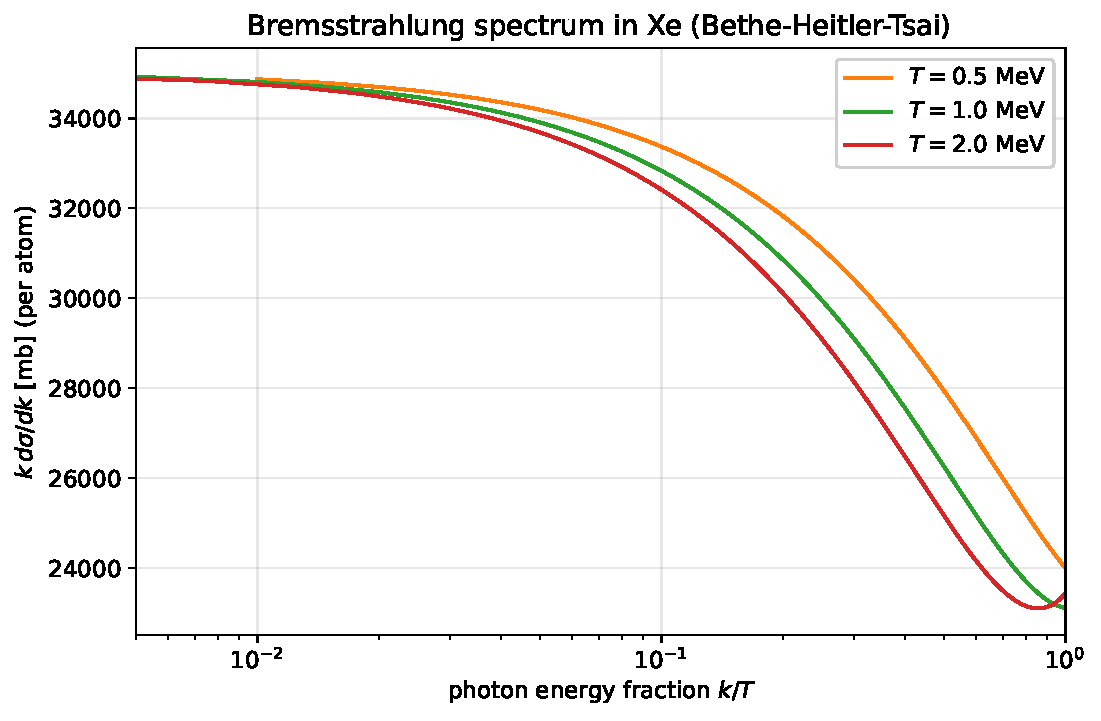
\includegraphics[width=0.72\textwidth]{figs/brems_spectrum.pdf}
\caption{Bremsstrahlung spectrum in Xe, plotted as
$k\,\dd\sigma/\dd k$ versus $k/T$ on a log axis. The $1/k$
infrared divergence of $\dd\sigma/\dd k$ becomes a finite
intensity per log $k$.}
\label{fig:brems}
\end{figure}

\subsection{Photon angle and threshold}

The bremsstrahlung photon polar angle is sampled from the same
Urban form~(\ref{eq:Urban}) used for the leptons in pair
production, with $\theta_\gamma=(\me/E_e)\,u$. Below an
infrared cutoff $\kmin$ the brems energy is added to the local
electron deposit; above $\kmin$ it is sampled discretely and
pushed onto the photon stack. We adopt $\kmin=\SI{50}{keV}$ as
discussed in \Cref{sec:thresholds}.

\section{Statistical methods}\label{sec:stats}

This section is a self-contained tutorial on the sampling
techniques used. All MC physics packages~--~{\sc Geant4},
{\sc EGS}, {\sc Penelope}, {\sc Mcnp}~--~rely on the same handful
of methods, applied to different cross sections.

\subsection{Sampling distance to next interaction}

If $\Sigma_{\rm tot}=n_{\rm at}\sigma_{\rm tot}$ is the macroscopic
cross section [cm$^{-1}$], the probability of no interaction in a
length $s$ is $\exp(-\Sigma_{\rm tot} s)$. Inverse-CDF gives:
\begin{equation}
\boxed{\;
  s = -\frac{\ln r}{\Sigma_{\rm tot}(\Eg)}
\;}
\qquad r\sim U(0,1).
\end{equation}
For the photon, $\Sigma_{\rm tot}$ is constant between
interactions, so this is exact. For the electron, $\Sigma_{\rm tot}$
depends on $T$ which changes along the track: the electron must
be \emph{stepped}.

\subsection{Sampling which process occurs}

Probabilities are proportional to partial cross sections:
\(P_i = \sigma_i/\sigma_{\rm tot}\). One uniform deviate together
with cumulative sums does the job (Algorithm~\ref{alg:proc}).

\begin{algorithm}
\caption{Sample which photon process occurs.}
\label{alg:proc}
\begin{algorithmic}[1]
  \State $r \gets \texttt{rng}()$
  \If{$r < P_{\rm C}$} \State \Return Compton
  \ElsIf{$r < P_{\rm C} + P_{\rm P}$} \State \Return pair
  \Else \State \Return photoelectric
  \EndIf
\end{algorithmic}
\end{algorithm}

\subsection{Inverse-CDF method}

For a probability density $f(x)$ with cumulative
$F(x)=\int_{-\infty}^x f$, drawing $x = F^{-1}(r)$ with $r\sim
U(0,1)$ produces samples distributed as $f$. We use this for the
exponential distance, the simple non-relativistic Sauter
photoelectron polar angle, and as building blocks below.

\subsection{Rejection sampling}

When the inverse CDF is awkward but $f(x) \le M$ on $[a,b]$:
\begin{enumerate}\itemsep=0pt
  \item Draw $x \sim U(a,b)$ and $u \sim U(0,1)$.
  \item Accept if $u\,M < f(x)$; else go to step 1.
\end{enumerate}
Acceptance probability is $\int f / [(b-a)M]$. The method is
inefficient if $f$ is very peaked. The cure is to bound
$f(x) \le M\,g(x)$ by an envelope $g$ that is itself easy to
sample; this is rejection from an envelope.

\subsection{Composition method}\label{sec:composition}

If $f(x)=\sum_k\alpha_k\,f_k(x)$ with weights $\alpha_k>0$
summing to unity, sample by
\begin{enumerate}\itemsep=0pt
  \item Choose $k$ with probability $\alpha_k$;
  \item Sample $x$ from $f_k$.
\end{enumerate}
Composition can be combined with rejection.

\subsection{Klein-Nishina sampling}

Following the EGS-style algorithm~\cite{ButcherMessel,EGS4,G4-PRM},
write the integrand of $\dd\sigKN/\dd\eps$ (where $\eps=\Egp/\Eg$,
range $[\eps_0,1]$, $\eps_0=\me/(\me+2\Eg)$) as
\(\dd\sigKN/\dd\eps \propto [1/\eps + \eps] \cdot
[1 - \eps\sin^2\theta/(1+\eps^2)]\),
which is a composition of two PDFs $f_1(\eps)\propto 1/\eps$ and
$f_2(\eps)\propto \eps$, multiplied by a rejection function
$g(\eps)\le 1$. Algorithm~\ref{alg:KN} is the result.

\begin{algorithm}
\caption{Sampling Klein-Nishina (after \cite{G4-PRM}).}
\label{alg:KN}
\begin{algorithmic}[1]
  \State $\eps_0 \gets \me/(\me+2\Eg)$
  \State $\alpha_1 \gets -\ln \eps_0$,
        $\alpha_2 \gets (1-\eps_0^2)/2$
  \Repeat
    \State draw $r,r',r''\sim U(0,1)$
    \If{$r < \alpha_1/(\alpha_1+\alpha_2)$}
      \State $\eps \gets \eps_0^{\,r'}$
    \Else
      \State $\eps \gets \sqrt{\eps_0^2 + (1-\eps_0^2)\,r'}$
    \EndIf
    \State $t\gets \me(1-\eps)/(\Eg\eps)$,
           $\sin^2\theta \gets t(2-t)$
  \Until{$g(\eps) = 1 - \eps\sin^2\theta/(1+\eps^2) \ge r''$}
  \State \Return $\eps$  \quad\Comment{$\Egp = \eps\,\Eg$}
\end{algorithmic}
\end{algorithm}

\subsection{Pair production sampling}

Below \SI{2}{MeV} we sample $\eps$ uniformly on $[\eps_0,1-\eps_0]$
(the differential is essentially flat there). Above, we use a
flat envelope and rejection against the $\eps^2+(1-\eps)^2$ shape;
the residual screening factor is also $\le 1$ over the
relevant kinematic region.

\subsection{Bremsstrahlung sampling}

For sampling $k$ from $\dd\sigma/\dd k$ above $\kmin$, we use a
$1/k$ envelope (which captures the infrared divergence) sampled by
\(k = \kmin(T/\kmin)^r\) with $r\sim U(0,1)$. Rejection weight is
the ratio of the BH-Tsai differential to the envelope.

\subsection{Step-size choice}\label{sec:step-size}

For the electron, $\Sigma_{\rm tot}$ changes along the track. We
use \emph{condensed-history} stepping with maximum step
\begin{equation}
  \Delta s_{\max} = f_{\rm range}\,R(T),
\end{equation}
$f_{\rm range}\sim 0.05$. At each step we
(i)~lose $\Delta E_{\rm col}=(\dd E/\dd x)_{\rm col}\,\Delta s$ as
continuous ionization deposit;
(ii)~sample whether a hard brems photon is emitted with probability
$P=\Sigma_{\rm brems}(T;\kmin)\,\Delta s$;
(iii)~advance the particle by $\Delta s$.
With $f_{\rm range}=0.05$ at $T=\SI{1}{MeV}$, $\Delta s\sim
\SI{0.1}{mm}$ in $\rm LXe$, both $\Delta E_{\rm col}/T$ and $P$
are well below 1, validating the linearization.


\section{The tracking algorithm}\label{sec:algo}

\subsection{The particle stack}

We adopt a \emph{stack-based} implementation. The simulation
maintains a single LIFO stack of \emph{tracks}, each carrying:
particle type ($\gamma$, $e^-$, $e^+$); kinetic energy (or $\Eg$);
position; direction unit vector; parent ID and generation counter.
Secondaries pushed at each interaction are popped immediately,
so the depth-first traversal keeps the working set small. (FIFO
would do equally well at our energies; for highly developed
showers depth-first is more memory-efficient. The
\verb|G4StackManager| has three stacks~--~urgent / waiting /
postponed~--~whose distinction matters only for very large
showers.)

\subsection{The main loop}

\begin{algorithm}[H]
\caption{Main tracking loop.}
\begin{algorithmic}[1]
  \State seed photon stack with primary
  \While{stack not empty}
    \State $t \gets$ pop
    \If{$t$ is gamma}
      \State \texttt{TRANSPORT\_PHOTON}($t$)
    \Else
      \State \texttt{TRANSPORT\_LEPTON}($t$)
    \EndIf
  \EndWhile
  \State \Return all energy deposits
\end{algorithmic}
\end{algorithm}

\subsection{Photon transport}

\begin{algorithm}[H]
\caption{\texttt{TRANSPORT\_PHOTON}.}
\begin{algorithmic}[1]
  \While{$\Eg \ge \Egcut$}
    \State $\sigma_{\rm C}, \sigma_{\rm P}, \sigma_{\rm Ph} \gets$
            \textsc{NIST XCOM}$(\Eg)$
    \State $\Sigma_{\rm tot}\gets n_{\rm at}(\sigma_{\rm C}+\sigma_{\rm P}+\sigma_{\rm Ph})$
    \State $s\gets -\ln(\texttt{rng}())/\Sigma_{\rm tot}$
    \State advance position by $s$ along $\hat n$
    \If{position outside detector} \State \Return \EndIf
    \State sample which process (Algorithm~\ref{alg:proc})
    \State call \texttt{DO\_COMPTON} / \texttt{DO\_PAIR} /
                \texttt{DO\_PHOTOELECTRIC}
    \If{pair or photoelectric} \State \Return \EndIf
  \EndWhile
  \State deposit residual $\Eg$ locally
\end{algorithmic}
\end{algorithm}

\texttt{DO\_COMPTON} samples $(\Egp,\theta)$ via
Algorithm~\ref{alg:KN}, updates the photon, and pushes a new
electron of energy $T_e=\Eg-\Egp$ onto the lepton stack with
direction from~(\ref{eq:phie}).

\texttt{DO\_PAIR} samples $\eps$ from~(\ref{eq:BH-diff}) and angles
from~(\ref{eq:Urban}), pushes both leptons onto the stack, flags
the positron for end-of-range annihilation, and consumes the photon.

\texttt{DO\_PHOTOELECTRIC} samples a shell, emits a photoelectron
with $T_e=\Eg-E_{\rm shell}$ and Sauter angles, pushes it onto
the lepton stack, and handles atomic relaxation: with probability
$\omega_K$ a $K_\alpha$ photon is pushed, otherwise an Auger
electron is deposited locally.

\subsection{Lepton transport}

\begin{algorithm}[H]
\caption{\texttt{TRANSPORT\_LEPTON} for a single $e^\pm$ track.}
\begin{algorithmic}[1]
  \While{$T \ge \Tcut$}
    \State pick $\Delta s$ subject to the step-size constraints
    \State $\Delta E_{\rm col} \gets$ \textsc{NIST ESTAR}$_{\rm col}(T) \cdot \rho \cdot \Delta s$
    \State deposit $\Delta E_{\rm col}$ at current position
    \State advance position by $\Delta s$
    \State $T \gets T - \Delta E_{\rm col}$
    \State $P_{\rm br} \gets \Sigma_{\rm brems}(T;\kmin)\Delta s$
    \If{$\texttt{rng}() < P_{\rm br}$}
       \State sample $k$, $\theta_\gamma$, push photon onto stack
       \State $T \gets T - k$
    \EndIf
  \EndWhile
  \State deposit residual $T$ locally
  \If{positron}
     \State emit two \SI{511}{keV} photons isotropic and back-to-back
  \EndIf
\end{algorithmic}
\end{algorithm}

\section{Thresholds and numerical parameters}\label{sec:thresholds}

\Cref{tab:thresholds} collects all numerical parameters with
recommended defaults.

\begin{table}[ht]
\centering
\caption{Recommended numerical parameters for the LXe simulation.}
\label{tab:thresholds}
\renewcommand{\arraystretch}{1.15}
\begin{tabular}{p{2.6cm} c p{8.8cm}}
\toprule
parameter & default & justification \\
\midrule
$\Egcut$ & \SI{10}{keV} & photon mfp at \SI{10}{keV} in $\rm LXe$
is below \SI{50}{\micro m}; below the K-edge photons interact
photoelectrically and deposit locally. \\
$\Tcut$  & \SI{50}{keV} & electron range at \Tcut is
$\sim\SI{30}{\micro\m}\ll\Delta z$. \\
$\kmin$  & \SI{50}{keV} & photons of $k\le\kmin$ have mfp
comparable to $\Delta z$ in $\rm LXe$; absorbed locally. \\
$f_{\rm range}$ & 0.05 & keeps $\Delta E_{\rm col}/T \ll 1$. \\
$\Delta s_{\rm floor}$ & \SI{10}{\micro\m} & avoid tiny steps. \\
$\Delta s_{\rm ceil}$  & \SI{1}{mm} & keeps brems
probability per step small. \\
Sandia max & \SI{500}{keV} & validity bound; above this
interpolate NIST XCOM directly. \\
\bottomrule
\end{tabular}
\end{table}

\begin{cautionbox}
The thresholds $\Egcut$, $\Tcut$, $\kmin$ are not independent of
$\Delta z$. Halving $\Delta z$ would halve $\kmin$ accordingly.
Always rerun the validation tests of \Cref{sec:validation} when
changing them.
\end{cautionbox}

\section{Channel-by-channel SS-mimic mechanism}\label{sec:ssmimic}

For ROI background events, each photon channel mimics SS through a
distinct mechanism. \Cref{fig:ssfaking} summarizes the first-
interaction branching for the two principal background lines.

\begin{figure}[ht]
\centering
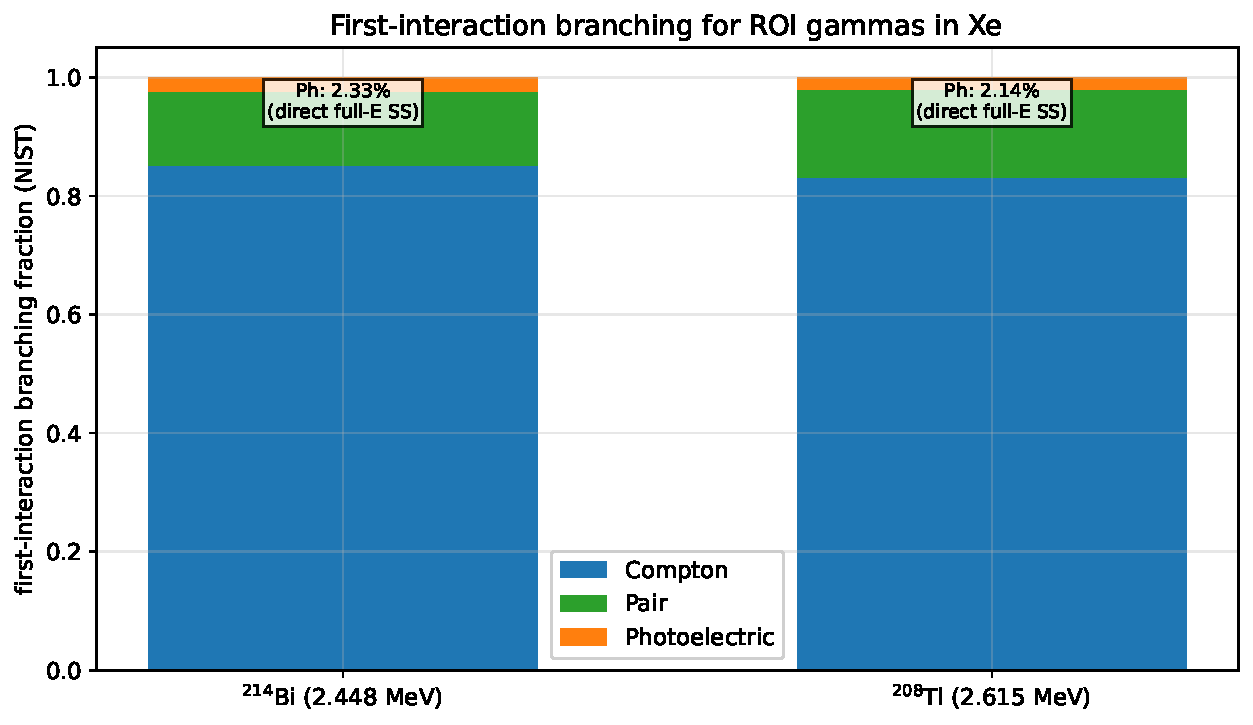
\includegraphics[width=0.78\textwidth]{figs/ss_faking_channels.pdf}
\caption{First-interaction branching for ROI gammas (NIST XCOM).
The photoelectric channel is small in branching but is the
direct full-energy SS-mimic: it deposits the full primary energy
at one point with $100\%$ probability of being SS.}
\label{fig:ssfaking}
\end{figure}

\paragraph{Photoelectric ($\sim 2\%$).} Direct full-energy
absorption at a single point. For $\rm{}^{214}Bi$ (energy
$\Eg=2.448$ MeV essentially in the ROI), \emph{every} photoelectric
event lands in the ROI and is SS, except for the tiny correction
from the K-shell fluorescence photon ($\SI{29.78}{keV}$, mfp
$\sim\!\SI{0.5}{mm}$) escaping the active volume from a near-edge
event. This makes photoelectric the most pernicious SS
background per interaction, even though it is the smallest
channel.

\paragraph{Compton ($\sim 85\%$).} The dominant first-interaction.
SS-mimic mechanism is a Compton chain followed by photoelectric
absorption of the residual scattered photon, all within $\Delta
z=\SI{3}{mm}$ of the first vertex. For $\rm{}^{208}Tl$ at
\SI{2.615}{MeV}, this requires the chain to deposit exactly
\SI{2.448}{MeV} (within ROI) and to do so in a localized way; the
typical SS fraction is $\sim 10$--$20\%$, depending on detector
geometry. \textbf{This is the channel where electron range and
bremsstrahlung corrections matter most}: bridging effects move
events from MS to SS, brems splitting moves them in the opposite
direction.

\paragraph{Pair ($\sim 13\%$).} Strongly biased \emph{against} SS:
the two annihilation \SI{511}{keV} photons travel typically
$\sim\!\SI{4}{cm}$ before depositing, almost guaranteeing MS
unless they both escape the detector or both interact within
$\Delta z$ of the primary vertex. SS-faking pair events are
rare but possible at the edge of the active volume; they
contribute to ROI background only at low rates.

The net SS fraction in the ROI is therefore the weighted sum
of these channel-specific mechanisms, with the photoelectric
channel contributing essentially $\sigma_{\rm Ph}/\sigma_{\rm tot}
\approx 2\%$ to the total SS-mimic rate from $\rm{}^{214}Bi$
\emph{independently of any topology corrections}.

\section{Validation tests}\label{sec:validation}

The simulation is validated by reproducing, on simple test cases:

\begin{enumerate}\itemsep=0pt
  \item \textbf{Total cross sections.} Sum-of-channels from NIST
        XCOM matches NIST total within $2.5\%$ (limited by log-log
        interpolation between sparse XCOM grid points).
  \item \textbf{Compton edge.} The Compton-electron sampler does
        not exceed $T_e^{\max}$, and the 99.9th percentile is
        within $1\%$ of the edge.
  \item \textbf{KN marginal.} The histogram of $\Egp$ from $10^5$
        sampled events at $\Eg=\SI{1}{MeV}$ agrees with the
        analytic Klein-Nishina differential to within $5\%$ in
        bulk bins.
  \item \textbf{Energy conservation.} For $5\times 10^2$ events at
        $\Eg=\SI{2.615}{MeV}$ in infinite $\rm LXe$, the mean
        energy lost (primary $-$ deposited) is below $10\,\text{keV}$,
        consistent with the threshold budget.
  \item \textbf{CSDA range.} The MC end-of-range for $T=\SI{1}{MeV}$
        electrons matches NIST ESTAR to better than $1\%$
        (no MS in our model: projected = CSDA).
  \item \textbf{Pair fraction.} For $\Eg=\SI{2.615}{MeV}$ primaries,
        the empirical first-interaction pair fraction agrees with
        NIST XCOM within statistical error.
  \item \textbf{511 keV peak.} A clear cluster at \SI{511}{keV} is
        produced by pair events (positron annihilation).
  \item \textbf{Hard-brems yield.} For \SI{2}{MeV} electrons, the
        sum of brems photon energies above $\kmin=\SI{50}{keV}$
        matches the expected hard-brems fraction of the NIST
        radiative yield to better than $40\%$.
  \item \textbf{SS fraction $\rm{}^{208}Tl$.} Run gives $\sim 10\%$
        in infinite $\rm LXe$, in agreement with literature
        $\sim 10$--$20\%$ for typical geometries.
\end{enumerate}

All nine tests pass in the distributed code (\verb|validation.py|).

\section{Comparison with \textsc{Geant4}}\label{sec:g4}

The {\sc Geant4} EM physics for the same problem is built around:
\begin{itemize}\itemsep=0pt
  \item Compton: \verb|G4KleinNishinaCompton|. Algorithm identical
        to ours (Algorithm~\ref{alg:KN}).
  \item Pair: \verb|G4BetheHeitlerModel|. Same differential as
        ours, sampled by composition + rejection.
  \item Photoelectric: \verb|G4LivermorePhotoElectricModel|
        (Livermore EPDL97 tabulated, not Sandia) is the modern
        default. Sandia is still available via
        \verb|G4PEEffectFluoModel|. We use Sandia below
        \SI{500}{keV} and NIST XCOM above; equivalent in accuracy
        to Livermore for our energy range.
  \item Bremsstrahlung: \verb|G4SeltzerBergerModel|, sampling $k$
        from the Seltzer-Berger tables by interpolation +
        rejection. We use the Bethe-Heitler-Tsai analytic form
        ($\sim 10\%$ accurate at our energies).
  \item Continuous ionization: \verb|G4eIonisation| with the
        Berger-Seltzer-equivalent ICRU-37 formula (this manual)
        and M\o{}ller cross section for $\delta$-rays (we omit
        $\delta$-rays).
  \item Multiple scattering: \verb|G4eMultipleScattering| with
        the Urban model~\cite{Urban2010} (we omit MS).
  \item Annihilation: \verb|G4eplusAnnihilation|, two-photon back-
        to-back at end-of-range (in our model too).
\end{itemize}

The differences are: no MS (few-tens-of-\% effect on projected
electron range; small effect on SS fraction); no $\delta$-rays
(negligible at $\Tcut=\SI{50}{keV}$); BH-Tsai brems instead of
Seltzer-Berger ($\sim 10\%$ on the differential); no Doppler
broadening (\order{1}~keV effect, irrelevant for SS/MS).

\begin{remarkbox}
\textbf{What you can borrow from {\sc Geant4} without porting it.}
The Seltzer-Berger tables ship as data files
(\verb|/data/G4EMLOW/brem_SB/|) in simple ASCII grids: read once
and interpolate. Sandia coefficients are similarly tabulated
(\verb|G4StaticSandiaData.cc|). Borrowing \emph{data} is much
safer than porting code.
\end{remarkbox}

\section{Physics we have chosen to omit}\label{sec:limits}

\begin{itemize}\itemsep=0pt
  \item \textbf{Doppler broadening of the Compton electron.} \order{1}
        keV effect on $T_e$; would matter only for sub-percent
        energy resolution.
  \item \textbf{Multiple scattering.} Replaced by straight CSDA
        segment; bias on projected end-of-range
        $\langle\cos\Theta\rangle\!\sim\!0.7$ is a known
        few-tens-of-\% systematic.
  \item \textbf{$\delta$-rays.} Negligible for our resolution.
  \item \textbf{Energy-loss straggling.} Smaller than detector
        resolution.
  \item \textbf{Rayleigh scattering.} Sub-percent of total
        attenuation; deposits no energy.
  \item \textbf{LPM effect.} Onset at $T\sim$~TeV; irrelevant.
  \item \textbf{In-flight positron annihilation.} $\sim\!1\%$;
        easy to add.
  \item \textbf{Three-photon ortho-Ps annihilation.} Branching
        $1/372$; negligible.
  \item \textbf{Photonuclear absorption.} Few percent in the
        giant-dipole region 5--30 MeV; outside our energies.
\end{itemize}

\section{Closing remarks}

The MC algorithm described here is intentionally minimal: the
smallest set of physics processes, sampling techniques, and
numerical parameters that can plausibly reproduce the SS/MS
classifier in a large LXe calorimeter to a few percent. The
exposition is meant as a launching pad for the reader who, having
understood every line, may then move to {\sc Geant4} or a refined
custom code \emph{knowing what each model means and which parts
matter}. We have shown that:
\begin{itemize}\itemsep=0pt
  \item the \textbf{photoelectric channel} ($\sim 2\%$ at our
        energies, \emph{not} per-mille) is small in branching
        but the most direct SS-mimic mode for $\rm{}^{214}Bi$;
  \item \textbf{electron transport with Bragg-like dE/dx and
        explicit bremsstrahlung} is essential for a quantitatively
        useful SS/MS estimate from Compton chains;
  \item \textbf{pair production} biases events toward MS via the
        two annihilation photons, reducing SS-mimic from $\rm{}^{208}Tl$.
\end{itemize}
The accompanying Python code reproduces these conclusions
end-to-end and can serve as a reference implementation for
extension.

\begin{thebibliography}{99}\small\itemsep=2pt
\bibitem{LZ} D.S. Akerib \emph{et al.} (LUX-ZEPLIN),
   \emph{Eur. Phys. J. C} \textbf{80} (2020) 1044.
\bibitem{nEXO} G. Adhikari \emph{et al.} (nEXO),
   \emph{J. Phys. G} \textbf{49} (2022) 015104.
\bibitem{EXO200} J.B. Albert \emph{et al.} (EXO-200),
   \emph{Phys. Rev. Lett.} \textbf{123} (2019) 161802.
\bibitem{NEXT} J.J. G\'omez-Cadenas \emph{et al.} (NEXT),
   \emph{Riv. Nuovo Cimento} \textbf{35} (2012) 29.
\bibitem{G4-1} S. Agostinelli \emph{et al.} (Geant4),
   \emph{Nucl. Instrum. Meth. A} \textbf{506} (2003) 250.
\bibitem{G4-PRM} Geant4 Collaboration,
   \emph{Geant4 Physics Reference Manual}, v11.4 (2024),
   \url{https://geant4.web.cern.ch/documentation/dev/prm_html/}.
\bibitem{KleinNishina} O. Klein, Y. Nishina,
   \emph{Z. Physik} \textbf{52} (1929) 853.
\bibitem{Hubbell1980} J.H. Hubbell, H.A. Gimm, I. \O{}verb\o{},
   \emph{J. Phys. Chem. Ref. Data} \textbf{9} (1980) 1023.
\bibitem{Urban1993} R. Brun \emph{et al.}, \emph{GEANT3 manual},
   CERN-DD-EE-84-1 (1993).
\bibitem{Urban2010} L. Urb\'an,
   \emph{Nucl. Instrum. Meth. A} \textbf{622} (2010) 314.
\bibitem{BiggsLighthill} F. Biggs, R. Lighthill,
   \emph{Sandia Lab.\ Report SAND87-0070} (May 1990).
\bibitem{Krause1979} M.O. Krause,
   \emph{J. Phys. Chem. Ref. Data} \textbf{8} (1979) 307.
\bibitem{ICRU37} ICRU Report 37, \emph{Stopping Powers for
   Electrons and Positrons} (1984).
\bibitem{Berger1964} M.J. Berger, S.M. Seltzer,
   \emph{NASA Report SP-3012} (1964).
\bibitem{Tsai1974} Y.S. Tsai,
   \emph{Rev. Mod. Phys.} \textbf{46} (1974) 815.
\bibitem{SeltzerBerger1985} S.M. Seltzer, M.J. Berger,
   \emph{Nucl. Instrum. Meth. B} \textbf{12} (1985) 95.
\bibitem{ButcherMessel} J.C. Butcher, H. Messel,
   \emph{Nucl. Phys.} \textbf{20} (1960) 15.
\bibitem{EGS4} W.R. Nelson, H. Hirayama, D.W.O. Rogers,
   \emph{The EGS4 Code System}, SLAC-265 (1985).
\bibitem{NIST-XCOM} M.J. Berger \emph{et al.}, NIST XCOM:
   \emph{Photon Cross Sections Database}, SRD~8 (2010),
   \url{https://physics.nist.gov/xcom/}.
\bibitem{NIST-ESTAR} M.J. Berger \emph{et al.}, NIST ESTAR:
   \emph{Stopping-Power and Range Tables for Electrons},
   SRD~124 (2005), \url{https://physics.nist.gov/Star/}.
\end{thebibliography}

\end{document}
